\documentclass[a4j,11pt,oneside,openany]{ltjsbook}
% SawareruSys User Manual (for SawareruSys v1.0.0)
% 2024-03-29 Naoki F., AIT. CC BY-SA 4.0 is applied.

\usepackage{amsmath}
\usepackage{graphicx}
\usepackage{here}
\usepackage{url}
\usepackage{ascmac}
\usepackage{txfonts}
\usepackage{geometry}
\usepackage{listings}
\usepackage{multirow}
\usepackage[ipaex]{luatexja-preset}

\geometry{truedimen,papersize={210truemm,297truemm}}
\geometry{top=30truemm,bottom=30truemm,left=20truemm,right=20truemm,footskip=10truemm}

\fboxsep=0pt
\fboxrule=1pt

\makeatletter
\def\linesperpage#1{\baselineskip=\textheight
  \divide\baselineskip by #1}

\renewcommand{\chapter}{%
  \if@openright\cleardoublepage\else\clearpage\fi
  \global\@topnum\z@
  \secdef\@chapter\@schapter}

\def\ps@plainfoot{%
  \let\@mkboth\@gobbletwo
  \let\@oddhead\@empty
  \def\@oddfoot{\normalfont\hfil-- \thepage\ --\hfil}%
  \let\@evenhead\@empty
  \let\@evenfoot\@oddfoot}
\let\ps@plain\ps@plainfoot
\makeatother

\pagestyle{plain}
\setcounter{secnumdepth}{3}
\setcounter{tocdepth}{2}

\lstset{numbers=left,frame=lines,basicstyle=\footnotesize\ttfamily,%
numberstyle=\footnotesize\itshape,xleftmargin=5truemm,escapeinside=||}
\let\origthelstnumber\thelstnumber
\makeatletter
\newcommand*\Suppressnumber{%
  \lst@AddToHook{OnNewLine}{%
    \let\thelstnumber\relax%
     \advance\c@lstnumber-\@ne\relax%
    }%
}

\newcommand*\Reactivatenumber[1]{%
  \setcounter{lstnumber}{\numexpr#1-1\relax}
  \lst@AddToHook{OnNewLine}{%
   \let\thelstnumber\origthelstnumber%
   \refstepcounter{lstnumber}
  }%
}
\makeatother

\title{{\Huge 「さわれる」遠隔学習システム}\\利用マニュアル}
\author{藤枝 直輝(愛知工業大学)}
\date{Version 1.0.0}

\begin{document}
\maketitle
\frontmatter
\tableofcontents
\mainmatter

% !TeX root=main.tex
\chapter{「さわれる」遠隔学習システムの概要}
%%%%%%%%%%%%%%%%%%%%%%%%%%%%%%%%%%%%%%%%%%%%%%%%%%%%%%%%%%%%%%%%%%%%%%%%%%%%%%
\section{システムの目的}

2019年末に発生した新型コロナウイルス感染症 (COVID-19) の拡大により,人同士の
接触を避ける観点から,本邦でもほとんどの大学で講義・実験の遠隔化,オンライン化
を迫られました.特に実験・実習科目においては,いかに実地での実験・実習と同等の
教育効果を遠隔環境で達成するかが,重要な課題となります.また,もしもそのような
システムがあれば,たとえ実地での実験・実習が可能である場合でも,実験時間外の
自主学習に活用できます.

しかしながら,ディジタル回路や FPGA の学習におけるこれまでの遠隔学習システム
には,その操作から実際にハードウェアに触れているとの実感を得ることが難しい,
という問題点がありました.例えば,ACRi ルーム \cite{ACRi_Room}上の仮想マシン
には FPGA ボードが接続されているものの,そのスイッチや LED 等を直接操作・確認
することはできませんでした.

我々(愛知工業大学 工学部電気学科 ディジタルシステム研究室)がこの問題点に対する
解決法として開発したのが,本マニュアルで説明する,ディジタル回路の「さわれる」
遠隔学習システムです.以下,本マニュアルではこのシステムを SawareruSys と表記
します.詳しい学術的背景や,システムの設計・評価については,文献
\cite{TALE-fujieda} を参照してください.

%%%%%%%%%%%%%%%%%%%%%%%%%%%%%%%%%%%%%%%
\section{必要な機材・ソフトウェア一式}

遠隔実験の実施には,FPGAボードの入出力の変化を手元で確認するためのコントローラ
ボードが必要です.2024年3月現在,コントローラボードには以下の3つのバリエーション
があります.

\begin{enumerate}
 \item FPGA リモコンボード V2
 \item FPGA リモコンボード V4
 \item SawareruBoard V1
\end{enumerate}

\begin{figure}[ht]
 \centering
 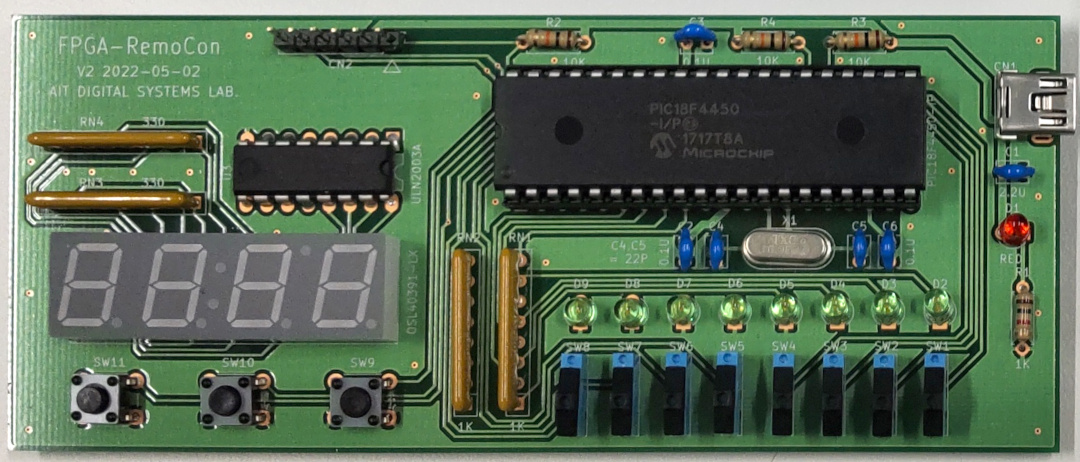
\includegraphics[width=80truemm]{figs/remocon_v2.jpg}
 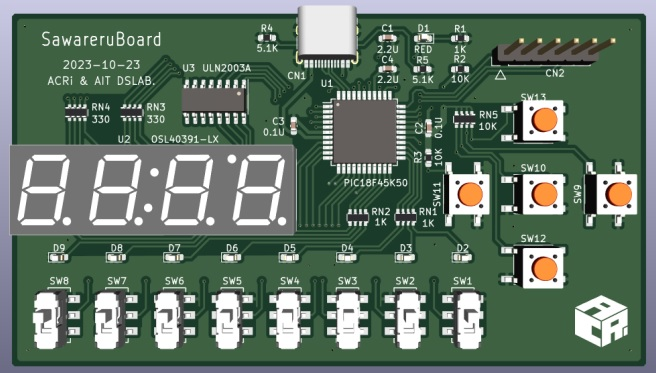
\includegraphics[width=60truemm]{figs/sawareru_v4.jpg}
 \caption{コントローラボードの例(左: FPGA リモコンボード V2,右: SawareruBoard V1).}
 \label{fig:boards}
\end{figure}

このうち1と3のボードの外景を,図\ref{fig:boards}に示します.
1のボードは,左・中央・右の3つのタクトスイッチを備え,PC との接続端子は USB
mini-B です.2と3のボードは機能的・形状的に同一で,十字型の5つのタクトスイッチ
を備え,接続端子は USB Type-C です.

また,SawareruSys の配布パッケージには,以下のファイル一式が含まれています.
\begin{itemize}
 \item DRFront: SawareruSys での開発を支援するためのフロントエンドツール
 \item Connectorアプリ: コントローラボードを遠隔サーバに接続するときに使用
 \item WinSCP: 遠隔サーバへファイルを転送するときに使用
\end{itemize}
加えて,Windows標準の以下のアプリケーションも使用します.
\begin{itemize}
 \item Windows PowerShell
 \item リモートデスクトップ接続
\end{itemize}

なお,WinSCP は Martin Prikryl 氏による著作物であり,GPL (version 3) ライセンス
に従って,ポータブル版の実行ファイルを再配布しています.ライセンスに関する詳細は,
配布パッケージの COPYING ファイルを参照してください.

%%%%%%%%%%%%%%%%%%%%%%%%%%%%%%%%%%%%%%%
\section{遠隔サーバの構成}

\begin{figure}[ht]
 \centering
 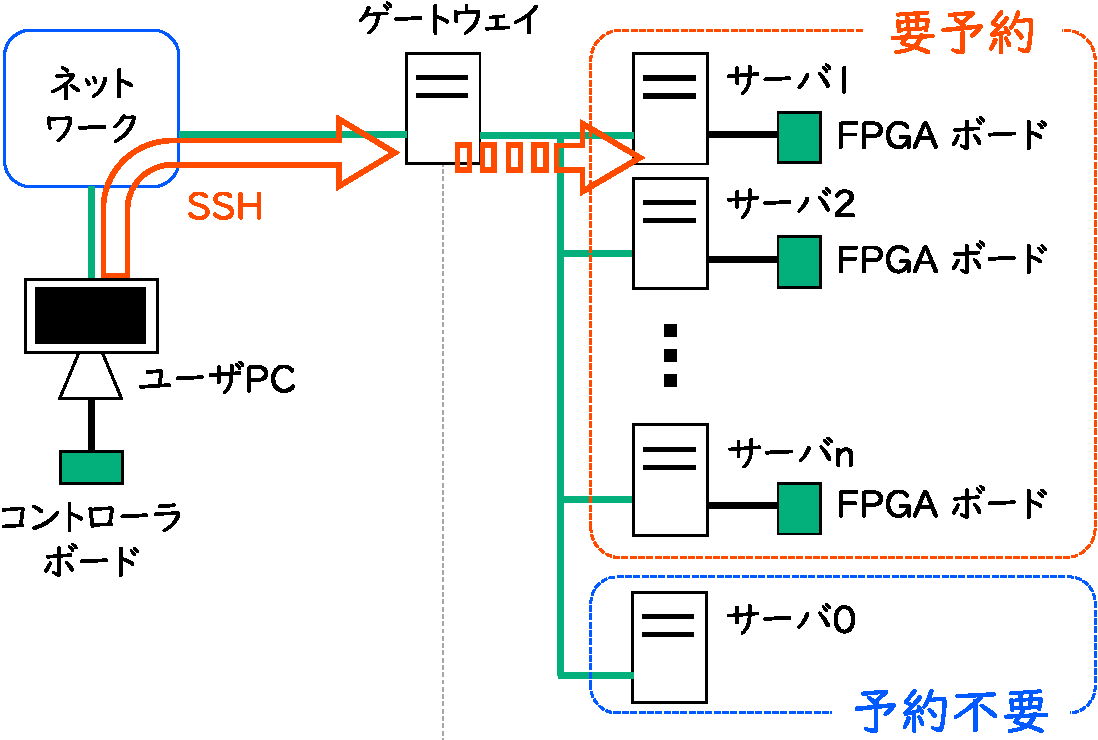
\includegraphics[width=80truemm]{figs/servers.pdf}
 \caption{遠隔サーバの構成図.}
 \label{fig:servers}
\end{figure}

SawareruSysにおける遠隔サーバの構成図を,図\ref{fig:servers}に示します.
遠隔サーバへの入口としてゲートウェイサーバが設置されており,ユーザは SSH 接続で
ゲートウェイサーバに接続します.開発用のサーバへのアクセスは,SSH ポートフォワー
ディング機能により間接的に行います.開発用のサーバには,FPGA ボードが1台ずつ設置
された予約の必要なサーバと,FPGA ボードが接続されていない予約不要のサーバとが
あります.

2024年3月時点の ACRi ルームでは,ゲートウェイサーバには fserv4,開発用のサーバには
vs000~vs910 の名前がつけられています.このうち末尾2桁が 00 であるサーバは予約不要
のサーバです.
愛工大の学内環境では,ゲートウェイサーバには gs1,開発用のサーバには ns0~ns5 の
名前がつけられています.ns0 は予約不要です.
予約が必要なサーバは,Web ブラウザで予約を行います.予約について詳しくは,各環境
のドキュメントまたは利用説明ページを確認してください.

PC と開発用のサーバでは,それぞれ別々の Connector アプリを起動して,通信の中継を
行います.PC とコントローラボード,サーバと FPGA ボードの通信には,それぞれで
USB-UART(USB を介したシリアル通信)を使用します.一方,PC とサーバとの通信は,
SSH ポートフォワーディングを介した TCP/IP 通信によります.このプロトコルの違いを
吸収し,通信の中継を行うのが,Connector アプリです.

%%%%%%%%%%%%%%%%%%%%%%%%%%%%%%%%%%%%%%%
\section{FPGA 内の回路構成}

SawareruSys では,入出力の遠隔操作を実現するために,FPGA 内部にあらかじめ入出力
制御回路を作りこんでおきます.ユーザは,入出力制御回路と接続されるユーザ回路部分
のみを開発します.

\begin{figure}[ht]
 \centering
 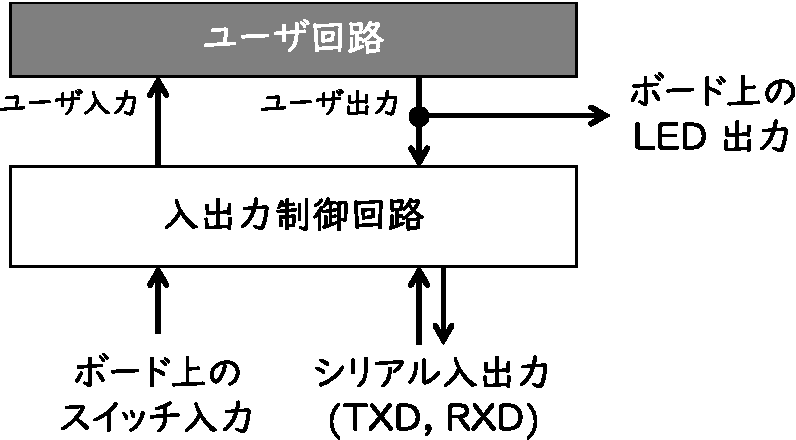
\includegraphics[width=80truemm]{figs/iocircuit.pdf}
 \caption{FPGA の内部構造の概要.}
 \label{fig:iocircuit}
\end{figure}

入出力制御回路とユーザ回路の関係の概要を,図\ref{fig:iocircuit}に示します.
入出力制御回路はシリアル通信の入出力(TXD と RXD)をもっており,サーバの
Connector アプリと接続されたかどうかや,入出力の変化の状況をチェックしています.
FPGAボードのスイッチ入力は,まず入出力制御回路に入ります.
サーバと接続されていない場合は,単にスイッチ入力の情報がユーザ回路の入力と
して渡されます.サーバと1度でも接続された場合は,入出力制御回路はコントローラ
ボードのスイッチの状態を受け取って保持し,その結果をユーザ回路の入力とします.
ユーザ回路の出力は,ボードの LED(または7セグメント LED)出力として使われる
ほか,入出力制御回路にも渡されます.
サーバと接続されている間,入出力制御回路はユーザ回路の出力の変化を監視し,
その結果をサーバに送ります.

SawareruSys では,ユーザ回路の入出力として,以下のものをサポートしています.
\begin{itemize}
 \item CLK: 100 MHz クロック 
 \item RST: リセットスイッチ(正論理)1 個
 \item SW(15)~SW(0): スライドスイッチ 16 個
 \item BTN{U, L, C, R, D}: タクトスイッチ 5 個(それぞれ,上,左,中央,右,下)
 \item LD(15)~LD(0): LED 16 個
 \item AN(7)~AN(0), CA~CG,DP: 7セグメント LED(負論理,8桁のダイナミック点灯)1 個
\end{itemize}
ただし,SW(15)~SW(8) はコントローラボードから操作できず,LD(15)~LD(8) と
7セグメント LED の左側4桁(AN(7)~AN(4) に対応)はコントローラボードから確認
できません.リセットスイッチは,ユーザ回路と入出力制御回路の両方をリセットします.
サーバと接続されていた場合には,接続されていない状態に戻りますので,ボードの
スイッチ入力が再び使えるようになります.

FPGA において,あらかじめ作りこまれた回路に自由に書き換えられるユーザ回路を
組み込んで使うための1つの方法に,動的部分再構成(DPR; Dynamic Partial
Reconfiguration)があります.AMD 社の FPGA における DPR 機能は,DFX(Dynamic
Function eXchange)とよばれます.DFX 機能を使うためには,同社の FPGA 開発環境
である Vivado 上で,多数のステップからなるスクリプトを実行する必要があります.
DRFront は,SawareruSys での DFX に必要な手順を自動化・効率化するために開発
されたフロントエンドツールです.

%%%%%%%%%%%%%%%%%%%%%%%%%%%%%%%%%%%%%%%
\section{サポートする FPGA ボード}

2024年3月現在,SawareruSys では Digilent 社の Nexys A7-100T,Arty A7-35T,
CMod A7-35T の3種類の FPGA ボードをサポートしています.

\subsection{Nexys A7-100T}

\begin{figure}[ht]
 \centering
 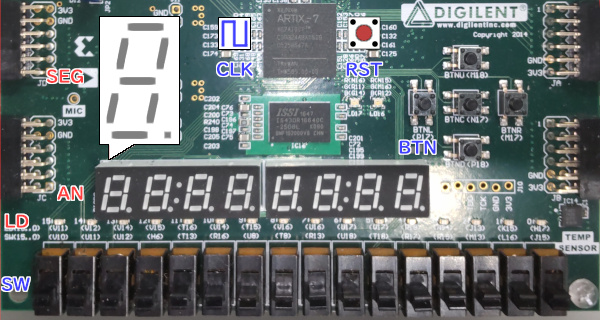
\includegraphics[width=90truemm]{figs/Nexys.jpg}
 \caption{Nexys A7-100T で使用できる入出力.}
 \label{fig:Nexys}
\end{figure}

Nexys A7-100T で物理的にアクセスできる入出力には,図\ref{fig:Nexys}に示す16個の
スライドスイッチ,5個のタクトスイッチ,16個のLED,8桁の7セグメント LED が含まれ
ます.これらすべてをユーザ回路上で扱えますが,スライドスイッチ・LED・7セグメント
LED のうち,左半分はコントローラボードでの確認・操作に対応していないことに注意
してください.リセットスイッチは,ボード右半分に2つ並んだ赤色のタクトスイッチ
のうち,左側のCPU RESET と書かれたスイッチです.

\subsection{Arty A7-35T}

\begin{figure}[ht]
 \centering
 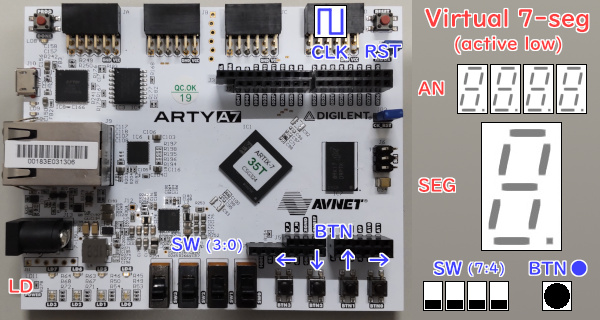
\includegraphics[width=90truemm]{figs/Arty.jpg}
 \caption{Arty A7-35T で使用できる入出力および仮想入出力.}
 \label{fig:Arty}
\end{figure}

Arty A7-35T は,Nexys A7-100T よりは安価なボードで,図\ref{fig:Arty}に示す
4個のスライドスイッチ,4個のタクトスイッチ(上下左右),8個のLEDに物理的に
アクセスできます.
LEDのうち4個は RGB LED ですが,SawareruSys では緑色の表示にのみ対応します.
コントローラボードを使って遠隔接続すると,仮想的に4桁の7セグメント LED と,
追加の4個のスライドスイッチ,1個のタクトスイッチ(中央)が利用できます.
リセットスイッチは,ボード右上の RESET と書かれたスイッチです.

\subsection{CMod A7-35T}

\begin{figure}[ht]
 \centering
 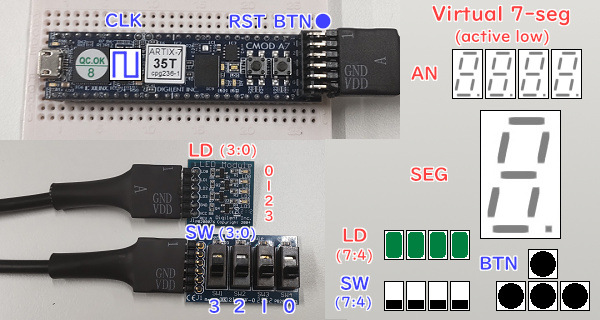
\includegraphics[width=90truemm]{figs/CMod.jpg}
 \caption{CMod A7-35T で使用できる入出力および仮想入出力.}
 \label{fig:CMod}
\end{figure}

CMod A7-35T は,ブレッドボードに差し込んで利用できる FPGA ボードで,サポートされて
いるボードの中では最も安価なボードですが,最小限の入出力装置しか備えていません.
そのため,Pmodケーブルキットの12ピン-デュアル6ピンケーブルを使用し,PMod 端子の
うち1~6ピンに PMod LED を,7~12ピンに PMod SWT を,それぞれ接続する使い方を
仮定します.接続例を図\ref{fig:CMod}に示します.あるいは,PMod 端子を使わずに,
ほぼすべてをコントローラボードから操作・確認する仮想入出力とみなすのもよいでしょう.

PMod 端子を使用した場合,CMod A7-35T を含む機材一式には,4個のスライドスイッチ,
1個のタクトスイッチ(中央),4個のLEDが含まれます.ボード上の2個のタクトスイッチ
のうち,ユーザ回路に接続されるのは右側のスイッチです.左側はリセットスイッチとして
使用します.コントローラボードを使って遠隔接続すると,4桁の7セグメント LED と,
追加の4個のスライドスイッチ,4個のタクトスイッチ(上下左右),4個の LED が仮想的
に利用できます.

PMod 端子を使用しない場合,CMod A7-35T には,1個のタクトスイッチ(中央)と3個の
LED が含まれます.ボード上の2個のタクトスイッチは,右側がユーザ回路に接続され,
左側がリセットスイッチとして使われます.
LEDのうち1個は RGB LED ですが,SawareruSys では緑色の表示にのみ対応します.
コントローラボードを使うと,4桁の7セグメント LED ,8個のスライドスイッチ,
追加の4個のタクトスイッチ(上下左右),5個の LED が仮想的に利用できます.

CMod A7-35T のボードに搭載されたオシレータの出力周波数は 12 MHz ですが,
SawareruSys ではこれをクロック生成回路(MMCM)で 100 MHz にしてから,ユーザ回路
および入出力制御回路に与えています.

%%%%%%%%%%%%%%%%%%%%%%%%%%%%%%%%%%%%%%%
% !TeX root=main.tex
\chapter{クイックスタート・ガイド}

本章では,コントローラボードと遠隔サーバのアカウントを入手した人が,コントローラ
ボードを使って回路の動作確認を最初に行うまでの間に必要な手順を説明します.

%%%%%%%%%%%%%%%%%%%%%%%%%%%%%%%%%%%%%%%%%%%%%%%%%%%%%%%%%%%%%%%%%%%%%%%%%%%%%%
\section{アカウントの確認とパスワードの変更}

\textbf{注: 既にパスワードの変更を済ませている場合,本節の作業は不要です.} \vspace*{1ex}

遠隔サーバのアカウントが発行されたら,まずは遠隔サーバにログインできるか確認し,
仮パスワードを自分で決めたパスワードに変更してください.遠隔サーバへのログイン
には PowerShell を使用しますが,PowerShellはデフォルト設定ではフォントの問題で
日本語が文字化けする場合があります.そのため,その対処を行ってから作業すること
をおすすめします.

Windows PowerShell をスタートメニューから開き,タイトルバーを右クリックして,
「プロパティ」を選択します.ダイアログの「フォント」タブから好みの日本語フォ
ントを選択して,OKボタンを押すと,設定が反映されます.

その後,ネットワーク(愛工大の学内環境を使う場合は,学内LAN)に接続されたPCで,
PowerShell から以下のコマンドを入力します.
\begin{verbatim}
    ssh 〈ユーザ名〉@〈接続先〉
\end{verbatim}
ssh のあとには半角スペースが必要であることに注意してください.例えばユーザ名が
\texttt{tu\_fujieda} であり,接続先が \texttt{gw.acri.c.titech.ac.jp}であれば,
入力するコマンドは,
\begin{verbatim}
    ssh tu_fujieda@gw.acri.c.titech.ac.jp
\end{verbatim}
となります.

初回に限り,接続しようとしているサーバの確認を求められるので,yes と入力します.
その後,パスワードの入力を求められるので,発行された仮パスワードを入力します.
このとき文字を入力しても画面上には何の反応もありませんが,それで正常です.

ログインに成功し,画面上に\texttt{〈ユーザ名〉: \$}などといったプロンプトが表示
されたら,\texttt{passwd}(環境によっては\texttt{yppasswd})と入力してパスワード
の変更を行います.
まず仮パスワードを1回入力し,自分で決めたパスワードを2回続けて入力します.
このときもやはり入力内容は画面に反映されませんので,打ち間違いに気をつけてください.
「パスワードは正しく更新されました」,あるいはそれに相当する英語のメッセージが表示
されたら,この段階では PowerShell は閉じても構いません.

%%%%%%%%%%%%%%%%%%%%%%%%%%%%%%%%%%%%%%%
\section{回路設計と必要なファイルの作成}

SawareruSys では,あらかじめ遠隔操作のためのベース設計の回路が用意されています.
ユーザは,その一部を各自で作成した回路に書き換えて使用します.作成した回路を
ベース設計に接続するための回路は,SawareruSys の一部である DRFront を用いて,
自動的に生成します.
回路を作成するためには,作成した回路の各入出力ポートが,FPGA ボードのどの信号に
接続されるかを指定する必要があります.この設定も DRFront の画面上で行います.

まずは配布パッケージの DRFront フォルダにある DRFront.exe 実行ファイルをダブル
クリックして,DRFront を起動します.
デフォルトではハードウェア記述言語(HDL)として VHDL を,FPGA ボードとして
Nexys A7-100T を使用する設定になっていますので,これ以外の言語やボードを使う
場合は,Settings ボタンから使用する言語を変更してください.また,自分の PC に
Vivado をインストールしている場合,インストール先とバージョンを指定すると,
このあとの論理合成と実装までの作業を自分の PC で行えます.
これらの設定は最初の起動時に1回だけ必要です.

作成した回路の HDL 記述を1つのフォルダにまとめておきます.このとき,フォルダ名
に日本語や半角スペースが含まれていると,Vivado の実行時に不具合が発生すること
がありますので,フォルダ名は英数字で作成するようにしてください.自分の PC で
Vivado を動作させる場合,親フォルダについても同様です.

最上段の「Source Dir.」の入力欄の横に「...」と書かれたアイコンがあるので,それを
クリックし,HDL 記述をまとめたフォルダを指定します.記述やディレクトリ名に問題が
なければ,その下の段の「Create Project」というボタンが押せるようになっているので,
このボタンをクリックします.
すると,Projectの項目が「project\_1」に変わり,ボード画像の下のテーブルに,
回路の入出力の一覧が表示されます.このときの様子を図\ref{fig:drfront1_1}に示します.

\begin{figure}[ht]
 \centering
 \fbox{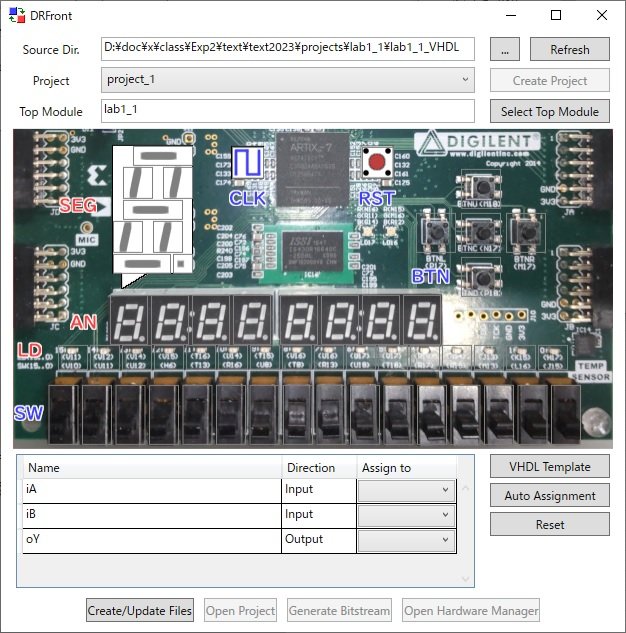
\includegraphics[width=70truemm]{figs/drfront1_1.jpg}}
 \caption{DRFront上でプロジェクトを作成したときの様子.}
 \label{fig:drfront1_1}
\end{figure}

なお,ファイルやディレクトリに問題があり入出力の信号が検出できなかった場合,
「Source Dir.」の入力欄が赤文字で表示されます.また,ディレクトリ名に日本語を
含んでいるなど,後々問題になりうる場合には,入力欄が黄色の背景で表示されます.
いずれもマウスカーソルを当てると問題点が表示されますので,それを参考にファイル
やフォルダ名,保存場所などを適切に修正してください.

入出力の設定には3通りの方法があります.
\begin{enumerate}
 \item 各信号の横の「Assign to」の列から,割当て先の信号を指定する.
 \item 信号名をドラッグして,ボード画像内の割当てたい部品へとドロップする.
 \item 自動割当てを使う.
\end{enumerate}

第1の方法では,「Assign to」の列をクリックすると,割当て可能な信号
(入力であればスイッチやボタン,出力であればLEDなど)の一覧が表示されます.
その中から割当てたい信号名を選ぶと,表の上側のボード画像の対応する部品を
囲む枠が水色で表示されます.これで割当ては完了です.
例として,入力信号iAを右端のスイッチ入力SW(0)に接続したときの様子を
図\ref{fig:drfront1_2}に示します.

\begin{figure}[ht]
 \centering
 \fbox{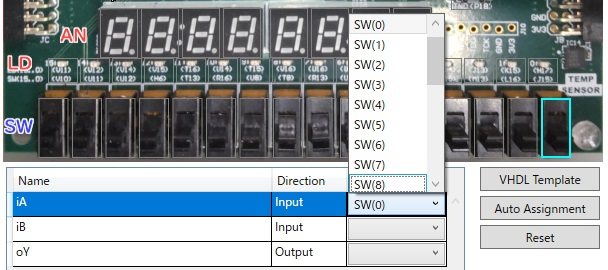
\includegraphics[width=80truemm]{figs/drfront1_2.jpg}}
 \caption{DRFront上で入力信号を割当てたときの様子.}
 \label{fig:drfront1_2}
\end{figure}

第2の方法では,割当てを行いたい信号の行をクリックして選択状態にしたあと,
マウスをドラッグしてボード画像上の割当てたい部品のところへと移動させます.
割当て可能であればマウスカーソルが切り替わり,枠が黄色で表示されるので,
そのままマウスボタンを離します(ドロップします).枠が水色で表示されれば,
割当て完了です.

第3の方法では,表の右側にある「Auto Assignment」ボタンをクリックします.
この方法では,まだ割当てが行われていない信号に対して,入力ならば
SW(0), SW(1), ... が,出力ならば LD(0), LD(1), ... を信号名の順に割当てます.
いくつかの信号を手動で割当てたあとで,自動割当てを行うこともできます.
各自の好みの方法で信号の割当てを行ってください.

すべての入出力への割当てが完了したら,DRFront の左下の「Create/Update Files」
ボタンを押します.すると,Vivadoの実行に必要なファイルが生成された旨が表示
され,「Open Project」ボタンが押せるようになります.

%%%%%%%%%%%%%%%%%%%%%%%%%%%%%%%%%%%%%%%
\section{必要なファイルの転送}

\textbf{注: 自分の PC に Vivado をインストールしている場合,先に2.6節の
「回路の論理合成と実装」の作業を行ってください.} \vspace*{1ex}

DRFront で必要なファイルが生成できたら,WinSCP を使ってそれらを遠隔サーバに
転送します.WinSCP を起動すると,セッション設定画面が表示されます.
転送プロトコルには SFTP または SCP,ホスト名には接続先のホスト名
またはIPアドレス,ユーザ名には遠隔サーバのユーザ名を入力します.
その後,必要に応じて保存ボタンで設定を保存してから,ログインボタンを押します.
SSH の場合と同様,ここでも最初に1回だけサーバの確認があるので,Yesと回答します.
パスワードの入力画面でパスワードを入力して,ログインしてください.

WinSCP のログイン後の画面では,通常左半分に自分のPCのファイル,
右半分に遠隔サーバ上のファイルが一覧表示されます.
ただし設定によっては,遠隔サーバ上のファイルのみが一覧表示される場合もあります.

まずは,遠隔サーバ上の適当な場所にフォルダを作成します.
このとき,Desktop フォルダ上で行うと,あとでリモートデスクトップ接続したときに
デスクトップにフォルダが表示されるので,見つけやすくなるかもしれません.
右半分の画面の適当な空欄を右クリックし,「新規」→「ディレクトリ」でフォルダ
を作成します.
次に,HDL 記述のあるフォルダを WinSCP の左半分の画面か,エクスプローラで開きます. 
フォルダ内にあるすべてのファイルとフォルダをドラッグし,WinSCP の右半分の画面上で
作成したフォルダにドロップすると,ファイル一式が転送されます.

ACRi ルーム上で初めてコントローラボードを使う場合には,2.9節で使用する Connector
アプリ(サーバ)も,このとき遠隔サーバに転送しておきます.配布パッケージの
Connector/Server フォルダにある connector\_serv.py を,遠隔サーバの適当な場所に
転送してください.愛工大の学内環境を使う場合はこの作業は不要です.

この時点で WinSCP は閉じても構いません.もし Vivado 実行後のプロジェクトを自分の
PC にダウンロードしたければ,WinSCP を開いたまま次の作業に進むこともできます.
遠隔サーバ上のファイル一覧は自動では更新されないので,Vivadoを実行するなどして
ファイルが更新されたと考えられる場合には,手動で更新ボタンを押してください.

また,自分のPC上のファイルと遠隔サーバ上のファイルは,自動では同期しないことにも
注意してください.もし記述ミスを見つけるなどして,自分のPC上のファイルを変更した
のであれば,そのファイルは忘れずに遠隔サーバにアップロードしてください.逆に,
遠隔サーバ上のリモートデスクトップでファイルを変更した際には,そのファイルを
遠隔サーバからダウンロードするのも忘れないでください.

ここまでの作業は,開発サーバを予約せずに進めることができます.
そのため,予約した時間が来るまでにここまでの作業を済ませておくと,動作確認が
円滑に進められるでしょう.

%%%%%%%%%%%%%%%%%%%%%%%%%%%%%%%%%%%%
\section{遠隔サーバへの接続}

予約した時間帯になったら,PowerShellを開き,sshコマンドを以下のとおり実行します.
\begin{verbatim}
    ssh -L 13389:〈サーバ名〉:3389 -L 13399:〈サーバ名〉:3399〈ユーザ名〉@〈接続先〉
\end{verbatim}
ただし,サーバ名は予約したサーバの名前,つまり vs + 数字3桁(ACRi ルーム),
または ns + 数字1桁(愛工大の学内環境)となります.
パスワードの入力を求められるので,遠隔サーバのパスワードを入力してログインします.
これにより,ゲートウェイサーバに接続するとともに,開発サーバへのポートフォワー
ディングの設定が行われます.

ログインが完了したら,リモートデスクトップ接続やコントローラボードの接続をして
いる間は PowerShell は開いたままにしておいてください.PowerShell を閉じると,
ポートフォワーディングの設定が解除されるため,リモートデスクトップやコントローラ
ボードも同時に切断されます.

毎回これを打ち込むのが面倒な場合には,上記のコマンドをメモ帳などに書き入れて,
拡張子 .ps1 で保存します.そのファイルを右クリックし「PowerShellで開く」を選択
すれば,自動でコマンドが実行されます.ただし,.ps1 ファイルを実行できない設定に
なっている場合は,以下のコマンドを PowerShell で実行して,実行可能な設定に変更
してください.
\begin{verbatim}
    Set-ExecutionPolicy RemoteSigned -Scope CurrentUser -Force
\end{verbatim}
なお,自分で作成したものでない .ps1 ファイルを安易に実行することはセキュリティ
リスクになりますので,十分注意してください.

%%%%%%%%%%%%%%%%%%%%%%%%%%%%%%%%%%%%
\section{リモートデスクトップ接続と Vivado の起動}

開発サーバ上で Vivado を実行したい場合には,Windows 標準のリモートデスクトップ
接続アプリケーションを使います.スタートメニューの「Windows アクセサリ」から
リモートデスクトップ接続を起動します.起動画面で「オプションの表示」をクリックし,
必要に応じて「画面」タブで画面サイズの設定を行ってください.「全般」タブで
「コンピューター」の欄に\texttt{localhost:13389}と入力して,「接続」ボタンを
押します.初回のみ「このリモートコンピュータのIDを識別できません」という
ウインドウが表示されるので,「このコンピュータへの接続について今後確認しない」を
チェックして,「はい」ボタンを押してください.

\begin{figure}[ht]
 \centering
 \fbox{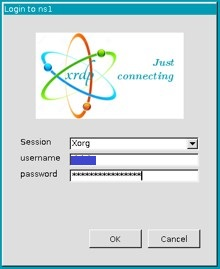
\includegraphics[width=60truemm]{figs/rdp_login.jpg}}
 \caption{開発サーバのログイン画面.}
 \label{fig:rdp_login}
\end{figure}

リモートデスクトップの画面では,最初に図\ref{fig:rdp_login}に示すログイン画面が
表示されます(ACRi ルームではユーザ名は自動入力されます).遠隔サーバのユーザ名
とパスワードを入力してログインします.正しくログインできれば,Ubuntu のデスク
トップ画面が表示されます.
デスクトップ画面が表示されたら,Ctrl+Alt+T キーを押すとターミナルが開きます.
開いたターミナル画面で以下のコマンドを入力すると,Vivado が起動します.
\begin{verbatim}
    source /tools/Xilinx/Vivado/2020.2/settings64.sh
    vivado &
\end{verbatim}
ただし,2020.2 のところは使いたいバージョンに合わせてください.愛工大の学内環境
では,この作業のかわりに,デスクトップに用意されたスクリプト start-vivado.sh を
ダブルクリックすることでも Vivado を起動できます.

%%%%%%%%%%%%%%%%%%%%%%%%%%%%%%%%%%%%
\section{回路の論理合成と実装}

本節の手順で,作成した回路をベース設計の回路と組み合わせて合成し,FPGA に書き込む
ビットストリームファイルを作成します.この作業は標準的には開発サーバ上の Vivado を
用いて行いますが,自分の PC に Vivado がインストールされている場合は,そこで作業
することもできます.

開発サーバ上の Vivado を用いる場合は,Vivado を起動したあと,必要な手順に対応する
スクリプトを読み込ませます.Vivado のメニューの「Tools」→「Run Tcl Script...」を
クリックし,プロジェクトのフォルダ(ソースのあるフォルダの直下に作成されている)
の中にある拡張子 .tcl のファイルを選択します.
自分の PC にインストールされた Vivado を用いる場合は,必要な手順に対応する DRFront
のボタンを押し,DRFront から Vivado を起動します.

\subsection{作成した回路の論理合成}

まずは,作成した回路そのものを論理合成します.開発サーバ上では,OpenProject.tcl を
読み込ませます.自分の PC では,DRFront の「Open Project」ボタンを押します.
10~20秒ほどすると,VHDLファイルのチェックが完了し,回路の階層関係が画面右上の
Sources タブに表示されます.Design Sources の下にあるDR\_TOPが,DRFront によって
作成されたベース設計との接続用の回路です.その横の「>」をクリックすると,この回路
に含まれる回路も表示されます.

階層関係の一例を,図\ref{fig:Vivado1_7_mod}に示します.この図は,DR\_TOP の中に
Deeds-DcSで作成した回路lab1\_1があり,さらにその回路がANDゲート(AND2\_gate)を
使用していることを示しています.

\begin{figure}[ht]
 \centering
 \fbox{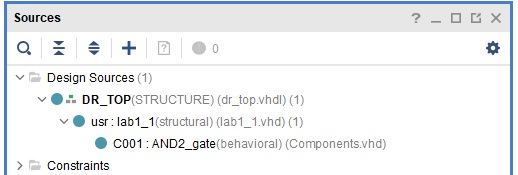
\includegraphics[width=80truemm]{figs/Vivado1_7_mod.jpg}}
 \caption{回路の階層関係表示の例.}
 \label{fig:Vivado1_7_mod}
\end{figure}

回路が無事認識されていることを確認したら,論理合成を行います.メニューの「Flow」
→「Run Synthesis」,または画面左側 Flow Navigator の「SYNTHESIS」→「Run
Synthesis」をクリックします.設定によっては論理合成の設定ダイアログが表示されま
すが,そのままOKボタンを押してください.数十秒ほど待つと論理合成が終了し,
図\ref{fig:Vivado1_8}で示すダイアログが表示されます.ここでは,Open Synthesized
Design を選択して OK ボタンを押し,論理合成結果を確認する画面を開いてください.

\begin{figure}[ht]
 \centering
 \fbox{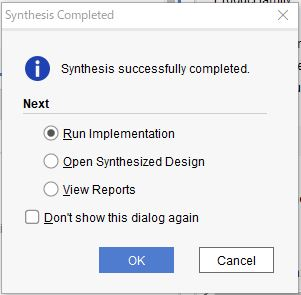
\includegraphics[width=60truemm]{figs/Vivado1_8.jpg}}
 \caption{論理合成成功のダイアログ.}
 \label{fig:Vivado1_8}
\end{figure}

なお,ダイアログを閉じてしまった場合や,論理合成結果を後から確認する必要がある
場合には,メニューの「Flow」→「Open Synthesized Design」または Flow Navigator
の「SYNTHESIS」→「Open Synthesized Design」をクリックすると,この画面に戻って
くることができます.

最後に,論理合成の結果をチェックポイントファイルとして保存します.メニューの
「File」→「Checkpoint」→「Write」から「Write Checkpoint」のダイアログを開き,
ファイル名を変更せずに OK を押します.自分の PC から Vivado を使用している場合,
この時点で Vivado は一旦閉じてしまっても構いません.開発サーバ上の Vivado では,
次のスクリプトを読み込ませると現在の作業内容は自動的に閉じられますので,Vivado
は開いたままで構いません.

\subsection{ベース設計との統合と実装}

ここから行う作業は,ベース設計に先ほど作成した回路を組込み,配置配線を行い,
ビットストリームとよばれるFPGAに書き込むためのデータファイルの作成を行う,
というものです.これらの一連の作業はすべてスクリプトで自動的に実行されます.

開発サーバ上では,GenerateBitStream.tcl を読み込ませます.自分の PC では,
DRFront の「Generate BitStream」ボタンを押します.すべての作業が終了するまでに
1~2分程度かかります.もしも途中でエラーが発生した場合には,Vivado はエラーの
内容を表示して停止します.問題なく全ての手順が完了した場合には,Vivado は
自動的に閉じ(あるいは起動直後の状態に戻り)ます.

本節で自分の PC を使って作業をしていた場合,ここで2.3節に戻り,必要なファイル
の転送とリモートデスクトップ上での Vivado の起動を行うことになります.次の手順
のために最低限転送する必要のあるファイルは,プロジェクトのフォルダの中にある
OpenHW.tcl と (回路名)\_(プロジェクト名).bit の2つのファイルです.

%%%%%%%%%%%%%%%%%%%%%%%%%%%%%%%%%%%%
\section{FPGA への書き込み}

FPGAに書き込むためのビットストリームファイルは,プロジェクトのフォルダの中に,
(回路名)\_(プロジェクト名).bit という名前で用意されます.動作試験前の最後の
手順は,FPGAへこのファイルを書き込むことです.開発サーバ上で起動している Vivado
に OpenHW.tcl を読み込ませます.Vivado が Hardware Manager 画面に切り替わります.
Hardware Manager では,図\ref{fig:Vivado1_12} に示す,まだハードウェアを開いて
いないという旨のメッセージが表示されます.

\begin{figure}[ht]
 \centering
 \fbox{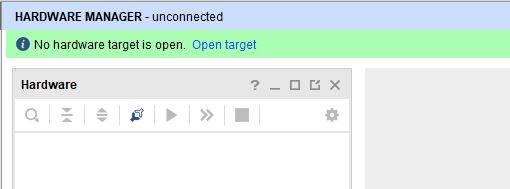
\includegraphics[width=70truemm]{figs/Vivado1_12.jpg}}
 \caption{Hardware Manager画面.}
 \label{fig:Vivado1_12}
\end{figure}

メッセージの横にある Open target のリンクをクリックし,Auto Connect を選択して,
サーバと FPGA との間の接続を行います.正しく接続できていれば,左上の Hardware
タブに (チップ名)\_0 というデバイスが表示され,画面が図\ref{fig:Vivado1_14} 
に示す通りに切り替わります.チップ名には,例えば xc7a100t などといった文字列が
入ります.

\begin{figure}[H]
 \centering
 \fbox{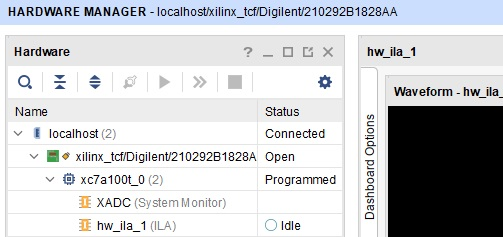
\includegraphics[width=70truemm]{figs/Vivado1_14.jpg}}
 \caption{Hardware ManagerでFPGAが認識されているときの様子.}
 \label{fig:Vivado1_14}
\end{figure}

(チップ名)\_0 を右クリックし,出てきたメニューから Program Device をクリック
すると,書き込むファイルを選択するダイアログが表示されます.「Bitstream file」
の入力欄の横にある「...」ボタンをクリックすると,図\ref{fig:Vivado1_15}に示す
ファイル指定のダイアログが表示されます.

\begin{figure}[H]
 \centering
 \fbox{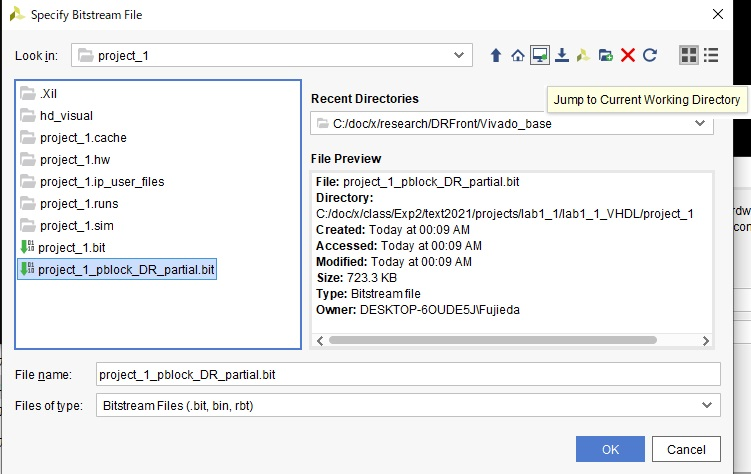
\includegraphics[width=70truemm]{figs/Vivado1_15.jpg}}
 \caption{書き込むビットストリームの選択画面.}
 \label{fig:Vivado1_15}
\end{figure}

ダイアログの右上の
\includegraphics[height=5truemm]{figs/Vivadoicon1_1.png}
のアイコンをクリックするとプロジェクトのディレクトリに移動します.そうすると,
書き込むべき .bit ファイルがファイルリストに現れますので,これを選択して OK 
ボタンを押します.最後に Program ボタンを押すと,ビットストリームが FPGA に
書き込まれ,作成した回路が動作を開始します.

ここまで開発サーバ上で Vivado を操作していた場合,Vivado 起動から FPGA への
書き込みまでの間に必要な手順は以下の通りとなります.

\begin{enumerate}
 \item Tool → Run Tcl Script で OpenProject.tcl を実行する
 \item Run Synthesis で論理合成を行う
 \item Open Synthesized Design で合成結果を開く
 \item File → Checkpoint → Write でチェックポイントを保存
 \item Tool → Run Tcl Script で GenerateBitstream.tcl を実行する
 \item Tool → Run Tcl Script で OpenHW.tcl を実行する
 \item Open target → Auto Connect でボードと接続する
 \item (チップ名)\_0 を右クリックして,Program Device を行う
\end{enumerate}

%%%%%%%%%%%%%%%%%%%%%%%%%%%%%%%%%%%%
\section{Connector アプリ(サーバ側)の準備}

\textbf{注: 愛工大の学内環境ではこの作業は不要です.Connector アプリが常時起動
する設定になっています.} \vspace*{1ex}

コントローラボードを使った動作確認のために,コントローラボードと FPGA ボードと
の間の通信を中継する Connector アプリを,サーバ側,PC 側の両方で起動します.
本節ではまずサーバ側の Connector アプリを起動します.

ターミナル上で2.3節で転送した connector\_serv.py のあるフォルダに移動します.
その上で,以下のコマンドで Connector アプリを起動します.
\begin{verbatim}
  python3 connector_serv.py /dev/ttyUSB1 3399
\end{verbatim}

Connector アプリが起動すると,動作ログがターミナル上に表示されます.FPGA
ボードが正しく認識できている場合,動作ログは例えば以下のような内容となります.
\begin{verbatim}
[2024-04-01 13:41:37] Connector for SawareruSys started.
[2024-04-01 13:41:37] Serial port opened.
[2024-04-01 13:41:37] Server started listening.
\end{verbatim}
Connector アプリを終了させたい場合には,Ctrl+C キーを押してください.

%%%%%%%%%%%%%%%%%%%%%%%%%%%%%%%%%%%%
\section{Connector アプリ(PC 側)の準備と動作確認}

つづいて,PC 側でも同様に通信の中継を設定します.PC 側で使用する Connector アプリ
は,配布パッケージの Connector/Client フォルダにある,Connector.exe 実行ファイル
です.

コントローラボードと PC を USB ケーブルで接続したあと,Connector アプリを起動
します.Controller Board の欄の下の None をクリックすると,その時点で接続されて
いるシリアル通信デバイスの一覧が表示されます.通常,コントローラボードは「USB
シリアル デバイス」という名前で認識されますので,その名前のついたデバイスを選択
してください.そうすると,Controller Board の欄下部の表示が,選択したデバイスの
ポート番号(COM + 数字)に切り替わります.FPGA ボード側のポート番号は,通常変更
する必要はありません.2.4節で遠隔サーバに接続したときに設定したポート番号(13399)
が自動で入力されています.Connector アプリでシリアル通信デバイスの一覧が表示
されているときの様子を,図\ref{fig:connector_port}に示します.

\begin{figure}[ht]
 \centering
 \fbox{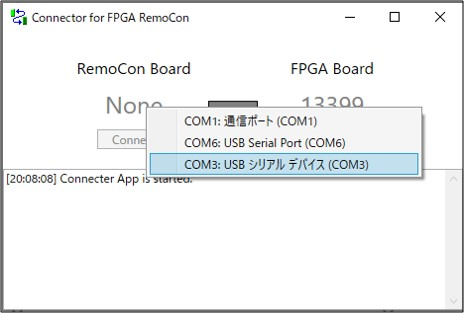
\includegraphics[width=60truemm]{figs/connector_port.jpg}}
 \caption{Connectorアプリのポート設定の例.}
 \label{fig:connector_port}
\end{figure}

ポート設定が済んだら,Connector アプリの両サイドの Connect ボタンを両方クリック
します.ボタン上の文字の色がともに青色に変わり,中央のバーの色が青色に変われば,
手元のコントローラボード,遠隔の FPGA ボードともに正しく認識されています.
この状態になれば,コントローラボードの入力を操作することで,FPGA ボードの入力を
遠隔で操作できるようになっているはずです.また,FPGA ボードの出力が,コントローラ
ボード上の LED や7セグメント LED で確認できるようになっているはずです.

%%%%%%%%%%%%%%%%%%%%%%%%%%%%%%%%%%%%
\section{接続を終了する前に}

動作確認をやめる場合には,まず PC 側の Connector アプリを終了して,コントローラ
ボードに接続された USB ケーブルを抜きます.リモートデスクトップ上では,Vivado と
サーバ側の Connector アプリを終了し,デスクトップ右上の電源マークのアイコンから,
「電源オフ/ログアウト」→「ログアウト」を選択して,開発サーバからログアウトします.

これらを確認してから,PowerShell を閉じて,遠隔サーバとの接続を終了してください.
PowerShell を先に閉じてしまうと,次回以降のログイン時に問題が生じる場合があります.

%%%%%%%%%%%%%%%%%%%%%%%%%%%%%%%%%%%%%%%%%%%%%%%%%%%%%%%%%%%%%%%%%%%%%%%%%%%%%%%
% !TeX root=main.tex
\chapter{コマンド体系}

本章では,コントローラボードと FPGA ボードとの間の通信に用いるコマンドについて
説明します.

%%%%%%%%%%%%%%%%%%%%%%%%%%%%%%%%%%%%%%%%%%%%%%%%%%%%%%%%%%%%%%%%%%%%%%%%%%%%%%
\section{コマンドの概要}

SawareruSys におけるコマンドは2つのASCII文字で1セットになっています.コマンドには,
(1) ボードの認識,(2) 出力,(3) 入力 の3種類があります.(1) は,コントローラボード
や FPGA ボードと,対応する Connector アプリとの間で主に使用します.(2) は FPGA
ボードからコントローラボードへと送信され,(3) はコントローラボードから FPGA ボード
に送信されます.Connector アプリは,(2) と (3) のコマンドに対しては中継のみ行います.

表\ref{table:command}に,現在定義されているコマンドを列挙します.コマンドの詳細は
3.2節以降を参照してください.

\begin{table}[hb]
 \centering
  \caption{コマンド定義の一覧表.}
  \label{table:command}
  \begin{tabular}{l|l|l} \hline
      & コマンド     & 定義 \\ \hline \hline
  (1) & V のあとに X & Connector アプリからのボード種別応答要求 \\
      & W のあとに Y & コントローラボードの種別応答 \\
      & v のあとに x & FPGA ボードの種別応答 \\
      & V のあとに Z & すべての入出力状態の再送要求 \\ \hline
  (2) & 0--4         & 出力グループの指定 \\
      & A--H/a--h    & 対応する出力をオン/オフにする \\ \hline
  (3) & I--S, q--r   & 入力の指定 \\
      & U/u          & 対応する入力をオン/オフにする \\ \hline
 \end{tabular}
\end{table}

%%%%%%%%%%%%%%%%%%%%%%%%%%%%%%%%%%%%%%%
\section{ボードの認識に関するコマンド}

ボードの認識に関するコマンドには4種類あります.第1のコマンドは ``VX'' の2文字で,
Connector アプリが接続されたボードに対して,ボードの種類を認識するために送信します.
コントローラボードは,コマンド ``VX'' を受け取ったら,第2のコマンドである ``WY''
で応答します.また,FPGA ボードは,第3のコマンドである ``vx'' で応答します.

Connector アプリはまた,ボードが動作しているかどうかを認識するために,``VX'' を
定期的に送信します.PC 側の Connector アプリはコントローラボードからの応答(``WY'')
を,サーバ側の Connector アプリは FPGA ボードからの応答(``vx'')を,それぞれ一定
時間内に受信できない場合は,タイムアウトとして接続を切断してもよいものとします.

第4のコマンドである ``VZ'' は,Connector アプリが,コントローラボードのすべての入力,
または FPGA ボードのすべての出力の状態を再送してほしいときに送信します.各ボードは,
すべての入力または出力に対してオン・オフのいずれかのコマンドを送信することで,この
コマンドに応答します.

%%%%%%%%%%%%%%%%%%%%%%%%%%%%%%%%%%%%%%%
\section{出力に関するコマンド}

コントローラボードには,8個の LED と4桁の7セグメント LED(小数点を含む)が搭載
されていますので,制御すべき LED の個数は $8 + (7 + 1) \times 4 = 40$ 個になります.
出力に関するコマンドでは,これを8つのセグメントからなるグループ5つで管理します.
コマンド文字列の1文字目では5つのグループいずれかを選択し,2文字目で8つのセグメント
のいずれかをオンまたはオフにします.

\begin{figure}[ht]
 \centering
 \fbox{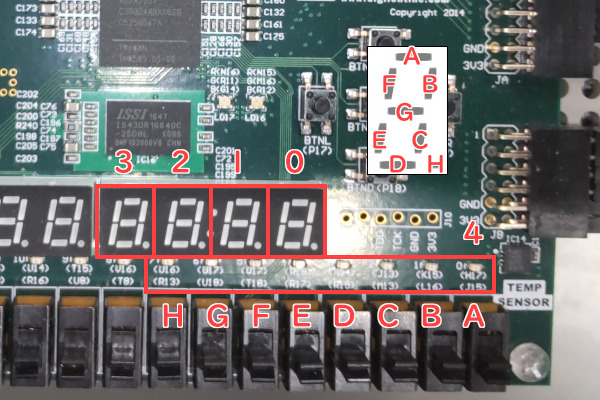
\includegraphics[width=80truemm]{figs/Nexys_LED.jpg}}
 \caption{出力グループおよびセグメントとコマンド文字の対応.}
 \label{fig:Nexys_LED}
\end{figure}

図\ref{fig:Nexys_LED}に,グループおよびセグメントと,対応するコマンド文字との対応を
示します.コントローラボードに図中に記載した文字 A--H のいずれかを送信すると,対応
するセグメントがオンになります.セグメントをオフにする場合には,小文字の a--h を
使用します.例えば,コマンド文字列 ``3G'' は,7セグメント LED の左端の桁の中央の
セグメントを点灯させる,という意味になります.

LED は,PWM 出力やダイナミック点灯により,しばしば頻繁にオン・オフされます.これらに
よって大量の通信が発生することを防ぐため,出力はサンプリングされています.詳細は
4章を参照してください.

%%%%%%%%%%%%%%%%%%%%%%%%%%%%%%%%%%%%%%%
\section{入力に関するコマンド}

コントローラボードには,8個のスライドスイッチと5個(または3個)のタクトスイッチが
搭載されています.入力に関するコマンドではこれらを個別に管理します.
コマンド文字列の1文字目では13個のスイッチいずれかを選択し,2文字目でそのスイッチを
オンまたはオフにします.

\begin{figure}[ht]
 \centering
 \fbox{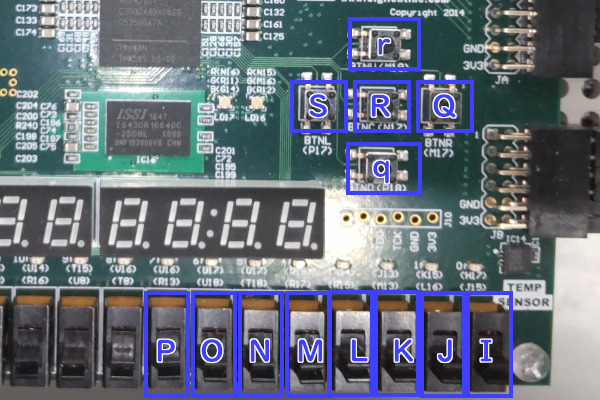
\includegraphics[width=80truemm]{figs/Nexys_SW.jpg}}
 \caption{入力とコマンド文字の対応.}
 \label{fig:Nexys_SW}
\end{figure}

図\ref{fig:Nexys_SW}に,スイッチと対応するコマンド文字との対応を示します.
FPGA ボードに図中に記載した文字 I--S または q,r のいずれかを送信したあと,U を送信
すると,対応するスイッチが仮想的にオンになります.スイッチをオフにする場合には,
小文字の u を使用します.例えば,コマンド文字列 ``SU'' は,左端のスライドスイッチを
オンにする,という意味になります.

%%%%%%%%%%%%%%%%%%%%%%%%%%%%%%%%%%%%%%%%%%%%%%%%%%%%%%%%%%%%%%%%%%%%%%%%%%%%%%
% !TeX root=main.tex
\chapter{入出力制御回路}

%%%%%%%%%%%%%%%%%%%%%%%%%%%%%%%%%%%%%%%%%%%%%%%%%%%%%%%%%%%%%%%%%%%%%%%%%%%%%%
\section{ベース設計の内部構造}

図\ref{fig:iodetail}に,より詳細なベース設計のブロック図を示します.ソースコード
は,パッケージの DRFront/BaseDesign\_RC フォルダに置かれており,図中の青字は回路名
またはソースコードのファイル名を示しています.青色白抜きで示している DR\_TOP が
ユーザ回路で,それ以外が入出力制御回路です.

\begin{figure}[ht]
 \centering
 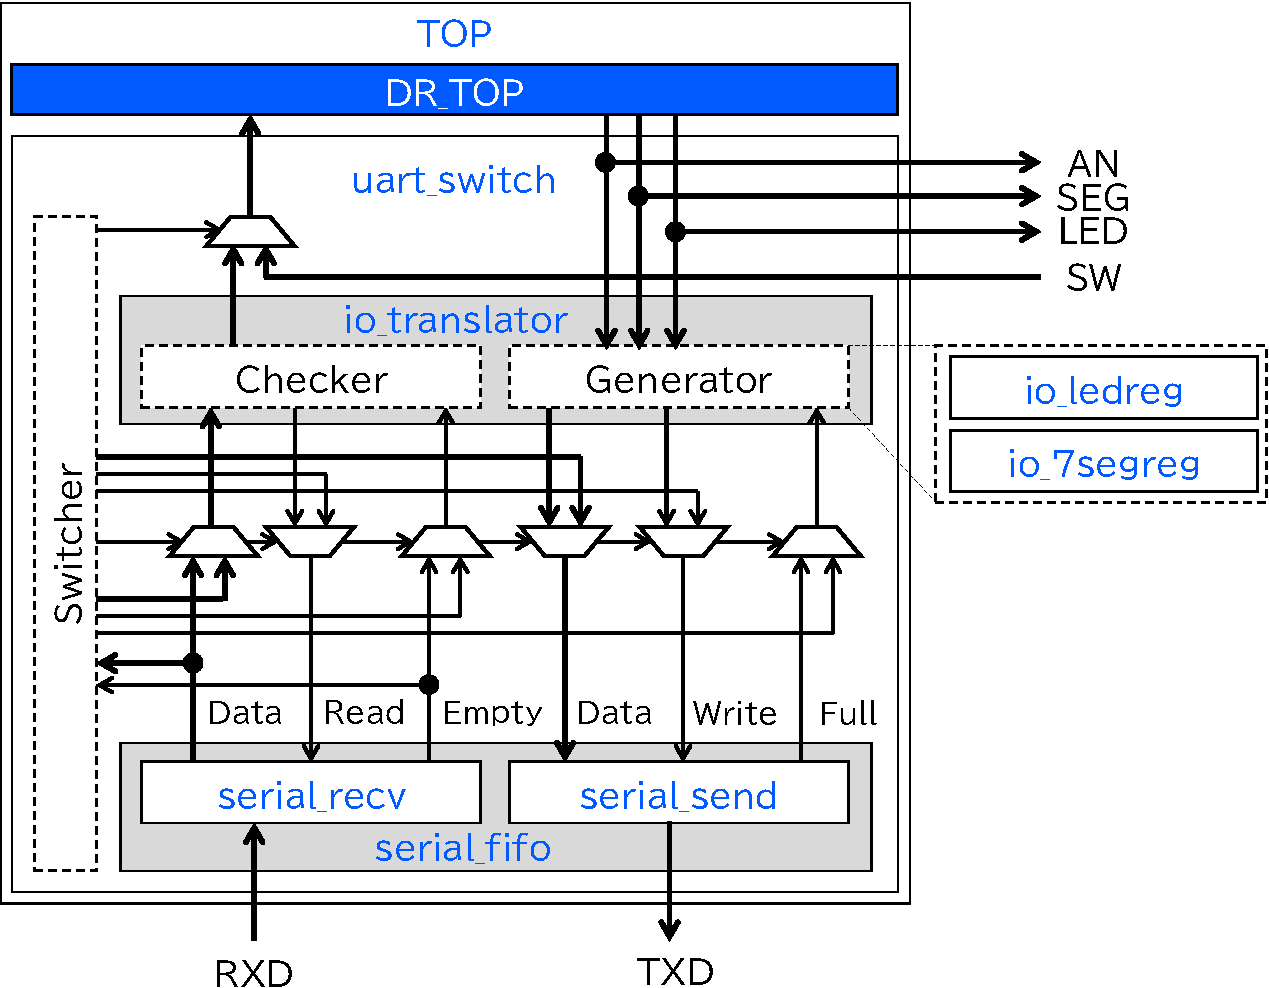
\includegraphics[width=110truemm]{figs/iodetail.pdf}
 \caption{ベース設計の内部構造.}
 \label{fig:iodetail}
\end{figure}

入出力制御回路には3つの主要な回路が組み込まれています.1つは UART コントローラ
(serial\_fifo),1つは I/O トランスレータ(io\_translator),もう1つはスイッチャー
回路(uart\_switch の内部回路)です.UART コントローラは,FPGA ボードの USB-UART
入出力に対するシンプルな FIFO インタフェースを提供します.I/O トランスレータは,
出力の生成回路(Generator)部分と入力のチェック回路(Checker)部分とに分かれて
います.

出力の生成回路部分では,コントローラボードが知っているであろう LED 出力の値を保持し,
現在のユーザ回路の出力と比較します.もし差異があれば,その中から1つを選択して,
コマンド文字列を生成するとともに,保持している LED 出力の値を更新します.

生成回路部分ではまた,出力のサンプリングも行っています.この目的は3つです.
第1の目的は,コマンドの生成される頻度を減らすことです.そのために,7セグメント
LED では 100 Hz で,通常の LED では 500 Hz で,それぞれ出力をサンプリングしています.
第2の目的は,通常ダイナミック点灯により制御される7セグメント LED の表示を安定
させるためです.そのために,サンプラーは7セグメント LED がどのように見えるかを
判定します.見た目が変わらない限りは生成回路部分からコマンドが送信されることは
ありません.第3の目的は,PWM 出力をおおまかに再現することです.ユーザが LED に
PWM 信号を与えていた場合,その周期がサンプリング周期と一致してしまうと,意図した
出力がコントローラボード上に得られないかもしれません.これを防ぐため,通常の LED
用のサンプラーは,単なるサンプリングではなく `1' が出力されていた割合をチェック
します.これが周期的に変化するしきい値よりも大きかった場合に,その LED 出力は `1'
であると判定します.

入力のチェック回路部分では,現在のスイッチ入力の値を保持し,コマンド文字列を待ちます.
スイッチをオン・オフするコマンド(`U' または 'u')を受信したら,対応するスイッチ
入力の値を `1' または `0' に変更します.

スイッチャー回路は,リセット直後は Connector アプリからの応答要求(``VX'')が送信
されるまで待機します.またこの間は,ボードのスイッチ入力をそのままユーザ回路へと
渡すとともに,I/O トランスレータからの信号をブロックします.これにより,FPGA
ボードが単体で動作している場合には,あたかもユーザ回路だけが動作しているかの
ように見えます.応答要求を受信したら,I/O トランスレータからの信号のブロックを
解除します.

%%%%%%%%%%%%%%%%%%%%%%%%%%%%%%%%%%%%%%%
\section{ベース設計の論理合成}

ベース設計の論理合成は,AMD FPGA の動的部分再構成(DFX)機能を使って行うため,
通常の論理合成とは方法が異なります.本節では,ソースコードからベース設計を論理合成
する手順を説明します.
なお,ソースコードの一部は対象とする FPGA ボードによって異なります.以降の説明では,
これを〈ボード名〉と表記します.ボード名は,Nexys,Arty,CMod のいずれかです.

\begin{enumerate}
 \item プロジェクトを新規作成し,ユーザ回路として空の回路を指定して,回路全体を
 論理合成します.設計のソースとして dr\_top.vhdl と 〈ボード名〉/dr\_base.vhdl
 \textbf{以外の}すべての VHDL ファイル,制約ファイルとして
 〈ボード名〉/〈ボード名〉.xdc を指定します.ロジックアナライザ(ILA)の IP コア
 設定として 〈ボード名〉/ila\_0.xci も設計のソースに追加します.
 \item 論理合成が終了したら,Open Synthesized Design で合成後の設計を開き,
 「File」→「Checkpoint」→「Write」でチェックポイントを保存します.保存したチェック
 ポイントファイルを,以後 step\_1.dcp とします.合成後の設計を開いた際に警告
 (Project 1-486)が表示されますが,無視して構いません.
 \item 別のプロジェクトを新規作成し,dr\_top.vhdl と 〈ボード名〉/dr\_base.vhdl
 を使って,デフォルトのユーザ回路を論理合成します.このとき,SYNTHESIS を右クリック
 して Synthesis settings を開き,More Options の欄に\texttt{-mode out\_of\_context}
 と入力します.これにより,不要な I/O バッファの挿入を抑止できます.
 \item 論理合成が終了したら,ステップ2と同様にチェックポイントを保存します.
 保存したチェックポイントファイルを,以後 step\_3.dcp とします.
 \item 「File」→「Checkpoint」→「Open」で step\_1.dcp を開きます.警告
 (Project 1-486)は無視して構いません.
 \item Tcl Console に以下のコマンドを打ち込み,ベース設計にデフォルトのユーザ回路を
 組み込みます.ただし,\texttt{/PATH/TO/CHECKPOINT} はチェックポイントを保存した
 フォルダのパス名とします.
\begin{verbatim}
    set_property HD.RECONFIGURABLE true [get_cells DR]
    cd /PATH/TO/CHECKPOINT
    read_checkpoint -cell [get_cells DR] step_3.dcp
\end{verbatim}
 \item ユーザ回路の配置される範囲(Pblock)を指定します.Vivado の画面右上 Device
 タブで,Draw Pblock のボタン(P+と書かれたアイコン)をクリックして,スライスや
 DSP,BRAM を含む適当な範囲を囲みます.
 \item 指定した Pblock の範囲に問題がないかチェックします.「Reports」→「Report DRC」
 を選択し,Rules で Dynamic Function Exchange にのみチェックを入れた状態で,DRC を
 実行します.もし DRC に失敗したら,エラーメッセージに従って Pblock の範囲を修正して,
 やり直してください.
 \item Tcl Console に以下のコマンドを打ち込み,作成した Pblock の範囲の設定を保存
 します.
\begin{verbatim}
    write_xdc -force PBLOCK.xdc
\end{verbatim}
 2回目以降は Pblock の範囲指定は \texttt{read\_xdc PBLOCK.xdc} で行えます.
 \item Tcl Console に以下のコマンドを打ち込み,実装とビットストリームファイルの作成
 を行います.
\begin{verbatim}
    opt_design
    place_design
    route_design
    write_bitstream -force -bin_file base.bit
    write_debug_probes -force base.ltx
\end{verbatim}
 \item Tcl Console に以下のコマンドを打ち込み,ユーザ回路を空の回路に戻した状態で
 チェックポイントを作成します.ここで作成したチェックポイントファイルを DRFront で
 使用します.
\begin{verbatim}
    update_design -cell DR -black_box
    lock_design -level routing
    write_checkpoint -force base.dcp
\end{verbatim}
\end{enumerate}

%%%%%%%%%%%%%%%%%%%%%%%%%%%%%%%%%%%%%%%%%%%%%%%%%%%%%%%%%%%%%%%%%%%%%%%%%%%%%%
% !TeX root=main.tex
\chapter{コントローラボード}

本章では,コントローラボードの仕様とコントローラボードのマイコン向けの制御プログラムの
ビルド方法,制御プログラムの書き込みと動作確認の方法について説明します.
なお本章では,「FPGA リモコンボード V2」を V2 ボード,「FPGA リモコンボード V4」および
「SawareruBoard V1」を V4 ボードと呼称します.

%%%%%%%%%%%%%%%%%%%%%%%%%%%%%%%%%%%%%%%%%%%%%%%%%%%%%%%%%%%%%%%%%%%%%%%%%%%%%%
\section{ボードの基本仕様}

コントローラボードは,USB に対応した PIC18F マイコンを搭載しています.マイコンの
型番は,V2 ボードが PIC18F4450-I/P(40ピン DIP),V4 ボードが PIC18F45K50/I-PT
(44ピン QFP)です.マイコンの汎用 I/O ピンとして使用できる全てのピンが,ボードの
入出力または USB の D+/D- 信号に割当てられています.表\ref{table:pic_io}に,入出力
の割当ての一覧を示します.入出力(名前は DRFront における表記に準拠)のそれぞれに
対して,割当て先となるマイコンのピン番号とポート名を記載しています.

\begin{table}[ht]
 \centering
  \caption{コントローラボードの I/O のマイコンへの割当て.}
  \label{table:pic_io}
  \begin{tabular}{c|c|l|c|l||c|c|l|c|l} \hline
   入力 & \multicolumn{2}{c|}{V2ボード} & \multicolumn{2}{c||}{V4ボード} &
   出力 & \multicolumn{2}{c|}{V2ボード} & \multicolumn{2}{c}{V4ボード} \\ \hline \hline
   SW(0) & 25  & RC6 & 17 & RB7 & LD(0) &  9  & RE1 & 26 & RE1 \\
   SW(1) & 26  & RC7 & 16 & RB6 & LD(1) &  8  & RE0 & 25 & RE0 \\
   SW(2) & 33  & RB0 & 15 & RB5 & LD(2) &  7  & RA5 & 24 & RA5 \\
   SW(3) & 34  & RB1 & 14 & RB4 & LD(3) &  6  & RA4 & 23 & RA4 \\
   SW(4) & 35  & RB2 & 11 & RB3 & LD(4) &  5  & RA3 & 22 & RA3 \\
   SW(5) & 36  & RB3 & 10 & RB2 & LD(5) &  4  & RA2 & 21 & RA2 \\
   SW(6) & 37  & RB4 &  9 & RB1 & LD(6) &  3  & RA1 & 20 & RA1 \\
   SW(7) & 38  & RB5 &  8 & RB0 & LD(7) &  2  & RA0 & 19 & RA0 \\
   BTNR  & 39  & RB6 & 32 & RC0 & AN(0) & 17  & RC2 &  5 & RD7 \\
   BTNC  & 40  & RB7 & 30 & RA7 & AN(1) & 16  & RC1 &  4 & RD6 \\
   BTNL  &  1  & RE3 & 18 & RE3 & AN(2) & 15  & RC0 &  3 & RD5 \\
   BTND  & n/a & n/a & 27 & RE2 & AN(3) & 10  & RE2 &  2 & RD4 \\
   BTNU  & n/a & n/a & 31 & RA6 & CA    & 19  & RD0 & 41 & RD3 \\
         &     &     &    &     & CB    & 20  & RD1 & 39 & RD1 \\
         &     &     &    &     & CC    & 21  & RD2 & 44 & RC6 \\
         &     &     &    &     & CD    & 22  & RD3 & 38 & RD0 \\
         &     &     &    &     & CE    & 27  & RD4 & 36 & RC2 \\
         &     &     &    &     & CF    & 28  & RD5 &  1 & RC7 \\
         &     &     &    &     & CG    & 29  & RD6 & 40 & RD2 \\
         &     &     &    &     & DP    & 30  & RD7 & 35 & RC1 \\ \hline
 \end{tabular}
\end{table}

電源 5 V は CN1 の USB ポート(mini B または Type-C)USB バスパワーで供給されます.
電源が供給されている間は,ボード上の D1 LED が赤色で点灯します.マイコンへの制御
プログラムの書き込みは,CN2 の ICSP 端子を介して行います.

コントローラボードのすべての入力は負論理です.またそのうち,マイコンの RB ポート
および RE3 ポートに接続されている入力については,マイコンの内部プルアップを使用
します.それ以外の入力は,10 k$\Omega$ の抵抗で明示的にプルアップされます.
一方で,コントローラボードのすべての出力は正論理です.通常の LED は 1 k$\Omega$の,
7セグメント LED は 330 $\Omega$ の抵抗により電流が制限されます.

%%%%%%%%%%%%%%%%%%%%%%%%%%%%%%%%%%%%%%%
\section{制御プログラムの書き込み}

制御プログラムのソースコードおよびプロジェクト一式は,PIC/RemoCon\_v?.x に置かれて
います.プログラムは MicroChip 社 MPLAB X IDE v6.10,MPLAB Code Configurator (MCC)
v5.3.7,および XC8 v2.4.1 を用いてビルドできることを確認しています.

V4 ボード向けの制御プログラムをビルドするためには,あらかじめ MCC によるコード再生成
が必要です.PIC/RemoCon\_v4.x フォルダを MPLAB X IDE 上でプロジェクトとして開くと,
プロジェクトに必要なファイルが見つからない旨のエラーが表示されます.このエラーは一旦
無視して,「Window」→「MPLAB Code Configurator v5」→「MPLAB Code Configurator v5:
Open/Close」で MCC を開きます.MCC で画面左上の Project Resources から,Generate
ボタンをクリックします.これにより,必要なファイルが自動的に生成されます.

制御プログラムがビルドできたら,PICkit などの PIC ライタを CN2 に三角の印を合わせて
接続して,プログラムをマイコンに書き込んでください.

書き込んだプログラムを簡易的に動作確認するためには,Tera Term などの UART に対応した
ターミナルアプリから,直接コマンドを打ち込みます.以下の手順で動作確認を行います.

\begin{enumerate}
 \item PC とコントローラボードを USB で接続します.
 \item ターミナルアプリでコントローラボードのシリアルポートを開きます.デバイス名は
 通常「USB シリアル デバイス」となります.転送レートは 115,200 bps,データは 8 bit,
 ストップビットは 1 bit,パリティとフロー制御はいずれもなしに設定します.
 \item ターミナルアプリ上で「VX」と入力すると,画面上に「WY」と表示されます.
 \item コントローラボードの左端のスライドスイッチをオン,オフと操作します.スイッチを
 オンにしたときとオフにしたときに,画面上にそれぞれ「PU」「Pu」と表示されます.
 \item ターミナルアプリ上で「3g」「3H」と入力します.7セグメント LED の左端の桁
 が消灯したあと,その桁の小数点が点灯します.
 \item ターミナルアプリ上で「4G」と入力すると,左端から2番目の LED が点灯します.
\end{enumerate}

%%%%%%%%%%%%%%%%%%%%%%%%%%%%%%%%%%%%%%%%%%%%%%%%%%%%%%%%%%%%%%%%%%%%%%%%%%%%%%

% !TeX root=main.tex
\chapter*{謝辞}
%%%%%%%%%%%%%%%%%%%%%%%%%%%%%%%%%%%%%%%%%%%%%%%%%%%%%%%%%%%%%%%%%%%%%%%%%%%%%%
SawareruSys は,日本学術振興会 科学研究費助成事業 基盤研究(C)課題番号 21K12164 
``ディジタル回路の「さわれる」遠隔学習システムに関する研究'' の支援により開発
され,その成果物として公開しているものです.

SawareruSys の開発および愛工大の学内でのテスト運用にあたっては,ACRi ルームの
運用ノウハウを大いに参考にしました.ACRi ルームの立ち上げに尽力された皆様,
特に東京工業大学の吉瀬謙二教授とイーツリーズ・ジャパンの三好健文氏に,厚く
御礼申し上げます.

また,いくつかの構成要素の開発にあたっては,愛工大ディジタルシステム研究室の
卒業生が下記の通り貢献しています.感謝申し上げます.

\begin{itemize}
 \item 原 瑛さん: 入出力制御回路の初期の開発
 \item 奥地 充稀 さん: Connector アプリのプロトタイプの構築
 \item 吉川 恵立 さん: Connector アプリのレイテンシ改善
\end{itemize}

%%%%%%%%%%%%%%%%%%%%%%%%%%%%%%%%%%%%%%%%%%%%%%%%%%%%%%%%%%%%%%%%%%%%%%%%%%%%%%

\nocite{*}
\bibliographystyle{junsrt}
\bibliography{main}

\appendix
%\include{A_VHDLsyntax}
%\include{B_remoteflow}
%\include{C_oldflow}

\end{document}